\documentclass{standalone}
\usepackage{tikz}
\usetikzlibrary{shapes}
\begin{document}
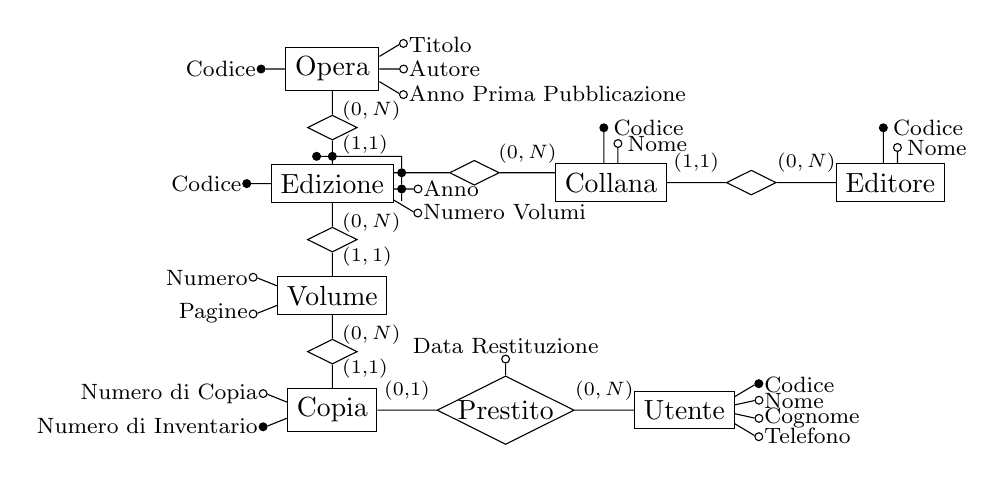
\begin{tikzpicture}
    \draw 

    % opera
    (0,0)node[draw, rectangle](opera){Opera}
    (opera.0)--++(0.25,0)node[draw, circle, inner sep=1pt,anchor=180]{}node[right]{\footnotesize Autore}
    (opera.15)--++(0.25,0.15)node[draw, circle, inner sep=1pt,anchor=195]{}node[right]{\footnotesize Titolo}
    (opera.345)--++(0.25,-0.15)node[draw, circle, inner sep=1pt,anchor=165]{}node[right]{\footnotesize Anno Prima Pubblicazione}
    (opera.180)--++(-0.25,0)node[draw, circle, inner sep=1pt, anchor=0, fill=black]{}node[left]{\footnotesize Codice}

    % edizione
    (opera.270)node[below right]{\scriptsize $(0,N)$}--++(0,-0.3)node[draw, diamond, shape aspect=2, inner sep=3pt, anchor=90](r1){}
    (r1.270)--++(0,-0.2)node[draw, circle, inner sep=1pt,fill=black](a){}--++(0,-0.1)node[above right]{\scriptsize (1,1)}node[draw, rectangle, anchor=90](edizione){Edizione}
    (edizione.355)--++(0.1,0)node[draw, circle, inner sep=1pt,fill=black](c){}--++(0.15,0)node[draw, circle, inner sep=1pt,anchor=180]{}node[right]{\footnotesize Anno}
    (edizione.345)--++(0.25,-0.15)node[draw, circle, inner sep=1pt,anchor=165]{}node[right]{\footnotesize Numero Volumi}
    (edizione.180)--++(-0.25,0)node[draw, circle, inner sep=1pt, anchor=0, fill=black]{}node[left]{\footnotesize Codice}
    
    % collana
    (edizione.10)--++(0.1,0)node[draw, circle, inner sep=1pt,fill=black](b){}--++(0.6,0)node[draw, diamond, shape aspect=2, inner sep=3pt, anchor=180](r3){}
    (r3.0)--++(0.7,0)node[midway, above]{\scriptsize $(0,N)$}node[draw, rectangle, anchor=170](collana){Collana}
    (collana.110)--++(0,0.45)node[draw, circle, inner sep=1pt, fill=black]{}node[right]{\footnotesize Codice}
    (collana.70)--++(0,0.25)node[draw, circle, inner sep=1pt, fill=white]{}node[right]{\footnotesize Nome}

    (a)++(-0.2,0)node[draw, circle, inner sep=1pt, fill=black](){}-|(b)--(c)--++(0,-0.15)

    % editore
    (collana.0)--++(0.75,0)node[midway, above]{\scriptsize (1,1)}node[diamond, draw, shape aspect=2, inner sep=3pt, anchor=180](r6){}
    (r6.0)--++(0.75,0)node[midway, above]{\scriptsize $(0,N)$}node[draw, rectangle, anchor=180](editore){Editore}
    (editore.110)--++(0,0.45)node[draw, circle, inner sep=1pt, fill=black]{}node[right]{\footnotesize Codice}
    (editore.70)--++(0,0.2)node[draw, circle, inner sep=1pt, fill=white]{}node[right]{\footnotesize Nome}
    
    % volume
    (edizione.270)node[below right]{\scriptsize $(0,N)$}--++(0,-0.3)node[draw, diamond, shape aspect=2, inner sep=3pt, anchor=90](r2){}
    (r2.270)--++(0,-0.3)node[above right]{\scriptsize $(1,1)$}node[draw, rectangle, anchor=90](volume){Volume}
    (volume.170)--++(-0.25,0.1)node[draw, circle, inner sep=1pt,anchor=350]{}node[left]{\footnotesize Numero}
    (volume.190)--++(-0.25,-0.1)node[draw, circle, inner sep=1pt,anchor=10]{}node[left]{\footnotesize Pagine}
    
    % copia    
    (volume.270)node[below right]{\scriptsize $(0,N)$}--++(0,-0.3)node[draw, diamond, shape aspect=2, inner sep=3pt, anchor=90](r4){}
    (r4.270)--++(0,-0.3)node[above right]{\scriptsize (1,1)}node[draw, rectangle, anchor=90](copia){Copia}
    (copia.170)--++(-0.25,0.1)node[draw, circle, inner sep=1pt,anchor=350]{}node[left]{\footnotesize Numero di Copia}
    (copia.190)--++(-0.25,-0.1)node[draw, circle, inner sep=1pt,anchor=10, fill=black]{}node[left]{\footnotesize Numero di Inventario}

    % utente
    (copia.0)--++(0.75,0)node[midway, above]{\scriptsize (0,1)}node[draw, diamond, shape aspect=2, anchor=180, inner sep=0.2pt](prestito){Prestito}
    (prestito.90)--++(0,0.15)node[draw, circle, inner sep=1pt, anchor=270]{}node[above]{\footnotesize Data Restituzione}
    (prestito.0)--++(0.75,0)node[midway, above]{\scriptsize $(0,N)$}node[draw, rectangle, anchor=180](utente){Utente}
    (utente.6)--++(0.25,0.055)node[draw, circle, inner sep=1pt,anchor=184]{}node[right]{\footnotesize Nome}
    (utente.356)--++(0.25,-0.055)node[draw, circle, inner sep=1pt,anchor=176]{}node[right]{\footnotesize Cognome}
    (utente.15)--++(0.25,0.15)node[draw, circle, inner sep=1pt,anchor=195, fill=black]{}node[right]{\footnotesize Codice}
    (utente.345)--++(0.25,-0.15)node[draw, circle, inner sep=1pt,anchor=165]{}node[right]{\footnotesize Telefono}
    
    ;
\end{tikzpicture}
\end{document}